\documentclass[11pt]{article}
\usepackage[letterpaper,margin=0.82in,headheight=15pt]{geometry}
\usepackage[T1]{fontenc}
\usepackage{lmodern,microtype}
\usepackage{amsmath,amssymb,amsthm,mathtools,booktabs}
\usepackage{graphicx,xcolor,caption,float}
\usepackage[colorlinks=true,linkcolor=tealblue,citecolor=tealblue,urlcolor=tealblue]{hyperref}
\definecolor{tealblue}{HTML}{087F8C}
\definecolor{ink}{HTML}{213547}
\definecolor{pale}{HTML}{EDF6F7}
\definecolor{quiet}{HTML}{657384}
\hypersetup{pdftitle={Surface envelopes versus the separated shortcut},pdfauthor={Method development report},pdfsubject={Accuracy audit and paired toy experiments for absolute and quantile residuals}}
\captionsetup{font=small,labelfont={bf,color=tealblue},skip=7pt}
\makeatletter
\renewcommand\section{\@startsection{section}{1}{\z@}{-2.8ex plus -1ex minus -.2ex}{1.3ex plus .2ex}{\large\bfseries\color{ink}}}
\renewcommand\subsection{\@startsection{subsection}{2}{\z@}{-2ex plus -.5ex minus -.2ex}{.8ex plus .2ex}{\normalsize\bfseries\color{ink}}}
\def\ps@research{\def\@oddhead{\small\color{quiet}Surface envelopes and the separated shortcut\hfil Research report}\let\@evenhead\@oddhead\def\@oddfoot{\small\color{quiet}Method audit \textbullet\ September 9, 2026\hfil\thepage}\let\@evenfoot\@oddfoot}
\makeatother
\pagestyle{research}
\setlength{\parskip}{4pt}\setlength{\parindent}{0pt}
\setlength{\textfloatsep}{13pt}\setlength{\intextsep}{12pt}
\emergencystretch=2em
\newtheorem{theorem}{Theorem}[section]
\newtheorem{lemma}[theorem]{Lemma}
\newtheorem{proposition}[theorem]{Proposition}
\newtheorem{remark}[theorem]{Remark}
\newcommand{\R}{\mathbb R}\newcommand{\E}{\mathbf E}
\newcommand{\tvec}{\mathbf t}\newcommand{\zvec}{\mathbf z}\newcommand{\evec}{\mathbf e}
\newcommand{\Q}{\mathcal Q_\alpha}\newcommand{\Cenv}{C_{\mathrm{env}}}\newcommand{\Cgwc}{C_{\mathrm{gwc}}}
\DeclareMathOperator{\cl}{cl}\DeclareMathOperator{\Rect}{Rect}
\newcommand{\takeaway}[1]{\par\vspace{4pt}\noindent\colorbox{pale}{\parbox{\dimexpr\linewidth-2\fboxsep\relax}{\small #1}}\par\vspace{4pt}}
\graphicspath{{figures/report_revision/}}
\begin{document}
\thispagestyle{empty}
{\small\bfseries\color{tealblue}METHODS \quad / \quad THEORY \quad / \quad REPRODUCIBLE EXPERIMENTS}\par
\vspace{12pt}
{\fontsize{25}{29}\selectfont\bfseries\color{ink}Surface envelopes versus\newline the separated shortcut}\par
\vspace{7pt}
{\large An accuracy audit and a paired toy-experiment study}\par
\vspace{6pt}
{\small\color{quiet}Absolute and quantile residuals \hfill September 9, 2026}\par
\vspace{13pt}
\begin{abstract}
\noindent
The surface-envelope construction tightens the old transductively standardized
conformal shortcut by bounding an entire location--scale ratio, rather than
separating its extrema. We recheck the construction, finite-sample proof,
signed inverse, search rule, and numerical boundary conventions, and add 2,400
fresh fitted trials spanning four noise distributions, calibration sizes,
and coverage targets. With identical nonnegative scores, the envelope is
uniformly weakly smaller in every coordinate while preserving marginal joint
validity. All new paired containment checks support that statement.
Signed quantile residuals offer additional gains but change the score
representation and do not have this uniform comparison. Timings also show
tradeoffs: speed depends on residual type and sample size. Nine figures connect
the proof to coverage, volume, coordinates, fixed-input geometry, and computation.
The complete mathematical development follows in the appendix.
\end{abstract}

\section{What ``uniform superiority'' means here}
For the same nonnegative residual function, calibration observations, target,
and compatible closed-cell conventions, the proved relationship is
\[
 C_{\rm full}(x)\subseteq C_{\rm env}(x)\subseteq C_{\rm old}(x),
 \qquad
 1-\alpha\le\Pr\{Y\in C_{\rm env}(X)\}\le\Pr\{Y\in C_{\rm old}(X)\}.
\]
Thus superiority means \emph{weakly smaller valid regions}. The smaller region
need not cover more test observations; on paired observations its coverage
cannot exceed that of its superset. Equality of some coordinates is allowed.
Neither strict improvement on every sample nor universal runtime dominance is
part of the result.

\takeaway{\textbf{Audit conclusion.} The core envelope argument remains valid.
This revision makes the old GWC comparison explicit, handles the projected
mean when GWC clips a coordinate, and separates mathematical guarantees from
floating-point implementation checks and empirical findings.}

In the primary six-outcome grid there are 1,440 paired fitted trials. No
coordinate containment violation occurs for either absolute or capped quantile
scores. All 1,440 absolute-volume pairs are finite; 1,342 capped pairs are
finite. Their equal-trial mean volume reductions are 3.14\% and 1.95\%,
respectively. The latter is conditional on a finite old volume, with 98
infinite-reference trials reported separately. These pooled numbers summarize
this grid; they are not distribution-free effect-size guarantees.

\clearpage
\section{The construction and its geometric meaning}
Write $m_j,s_j$ for the calibration mean and population-divisor standard
deviation, and let $N=n+1$. Adding a candidate coordinate $z$ gives
\[
 \mu_j(z)=\frac{nm_j+z}{N},\qquad
 \sigma_j(z)=\sqrt{s_j^2+(z-m_j)^2/N},\qquad
 F_j(t,z)=\frac{t-\mu_j(z)}{\sigma_j(z)}.
\]
On an active cell $I_j$ and off-coordinate GWC domains $G_\ell$, the envelope
uses the exact surface score
\[
 \max\!\left\{\sup_{z\in I_j}F_j(t_j,z),\;
                  \max_{\ell\ne j}\sup_{z\in G_\ell}F_\ell(t_\ell,z)\right\}.
\]
The old shortcut instead bounds $t/\sigma-\mu/\sigma$ by extrema that may
occur at different candidates. For $t\ge0$, this separation can only increase
the surface upper bound. Order-statistic monotonicity and the increasing
self-score inverse carry the inequality through to coordinate thresholds.
The detailed proof and all endpoint conditions appear in
Appendix~\ref{sec:dominance}.

\begin{figure}[H]\centering
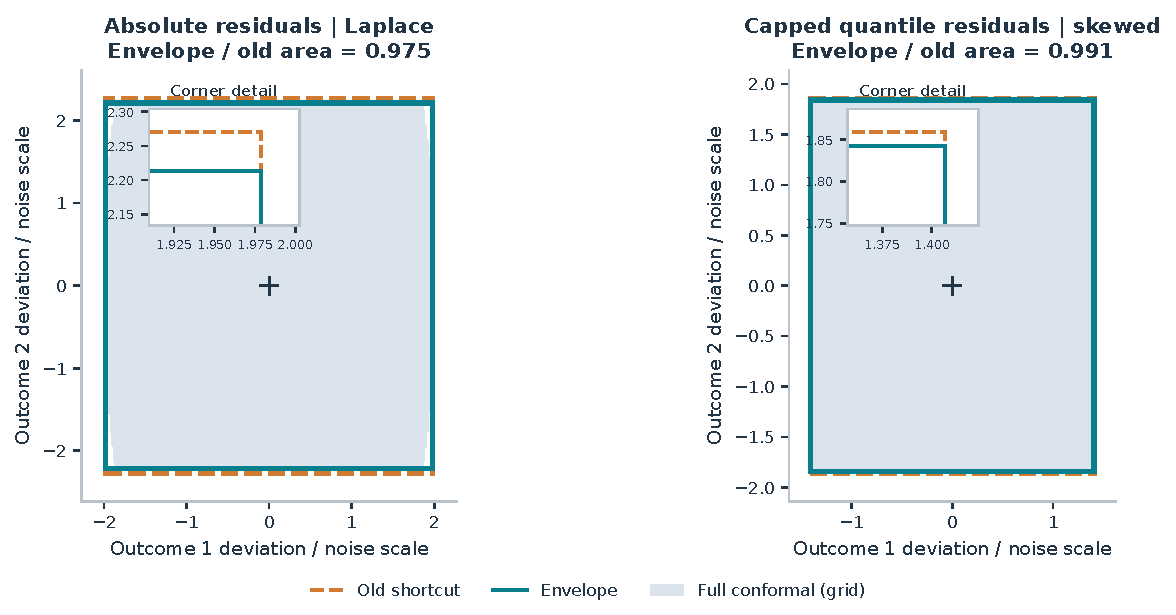
\includegraphics[width=\linewidth]{fixed_point_geometry.pdf}
\caption{\textbf{One input, two residual constructions.} Each panel uses a
fresh fitted two-outcome toy, $n=30$, trial 0 and test input 0, fixed before
plotting. The dashed old boundary encloses the envelope. Insets show the
small boundary differences without enlarging them in the main axes. Gray
marks full-conformal acceptance evaluated on a $241\times241$ outcome grid;
all 85,000 accepted grid candidates lie inside the envelope. Grid shading
illustrates geometry and is not an exact volume or coverage estimate. Axes
are centered at the fitted point prediction (left) or quantile midpoint
(right), and divided by each coordinate's known DGP noise scale.}
\label{fig:geometry}
\end{figure}

The envelope encloses accepted coordinate pieces; it can fill gaps and need
not equal the full-conformal set. Here the respective area ratios are 0.975
and 0.991. The examples are deliberately fixed, so they also convey that a
valid gain can be visually modest. The endpoint scale normalization is only
for display and leaves area ratios unchanged.

\clearpage
\section{Experimental design and estimands}
Every trial generates independent training, calibration, and test observations
and refits the models. Methods within a trial share all observations and fitted
predictions. There is no reused simulation pool or fitted model across trials.
We use 800 training and 1,200 test observations, three Gaussian features, and
six outcomes unless specified otherwise.

Let $g(x)=\mathbf1\{x_1>0\}$, $a_j$ be geometrically spaced from 0.6 to 2.4,
and $B_{kj}=\tfrac12\sin(\ell_{kj}+1)$, where $\ell_{kj}$ is the zero-based
row-major index in a $3\times d$ matrix. The data-generating model is
\[
 X\sim N(0,I_3),\qquad
 Y_j=X^\top B_{\cdot j}+(1+0.8g(X))a_j\epsilon_j.
\]
The four noise laws are independent standard Gaussian; Gaussian with
equicorrelation 0.8; independent unit-variance Laplace; and independent
centered, unit-variance $\exp(0.8Z)$ with $Z\sim N(0,1)$. Thus every family
includes covariate-dependent scale and heterogeneous outcome units, and the
last adds skewness.

\paragraph{Fitted absolute and quantile scores.}
An OLS model with intercept supplies $\hat f_j$. For each group and outcome,
the empirical training-error quantiles at $\beta/2$ and $1-\beta/2$ supply
offsets to $\hat f_j$, yielding ordered $\hat q_j^-,\hat q_j^+$.
This is a simple fitted location model with groupwise empirical quantile
offsets, not an oracle quantile model or a gradient-boosted quantile regressor.
All offsets are estimated from training data alone. With $w_j=\hat q_j^+-\hat q_j^-$:
\[
 E_j^{\rm abs}=|Y_j-\hat f_j(X)|,\qquad
 E_j^{\rm raw}=\max(\hat q_j^-(X)-Y_j,Y_j-\hat q_j^+(X)),\qquad
 E_j^{\rm cap}=\max(E_j^{\rm raw},0).
\]
The raw score and possible contraction of a fitted base interval follow the
CQR construction of Romano et al.~\cite{romano2019}. Here their coordinate
scores are used inside the audited multivariate envelope. Raw scores have
test-specific lower endpoint $-w_j(x)/2$. The old shortcut is evaluated on
absolute or capped scores; raw signed scores are not fed into its
nonnegative-score formula.

\paragraph{Prespecified grids.}
The primary grid crosses four noise laws with $n\in\{30,80,200\}$ at
$\alpha=\beta=0.1$, with 120 trials per cell (1,440 trials). At $n=80$,
Gaussian and Laplace toys additionally use $\alpha\in\{0.05,0.2,0.3\}$
(720 trials). Two Gaussian, two-outcome studies at $n=80$ use
$\beta\in\{0.1,0.02\}$ and $\alpha=0.1$ (240 trials).
Two further fitted datasets supply Figure~\ref{fig:geometry}; they are not
included in the Monte Carlo summaries.

\paragraph{Coverage, size, and uncertainty.}
Joint coverage is the within-trial proportion covering all outcomes.
Lengths are $2L_j$ for absolute scores and $w_j(x)+2L_j$ for quantile scores;
volumes are products of outcome lengths, averaged over the trial's test inputs.
Empty boxes have zero volume. We plot the mean of the \emph{paired trial ratios}
$V_{{\rm env},b}/V_{{\rm old},b}$, not a ratio of pooled mean volumes.
Ratios use finite positive denominators and finite numerators; excluded counts
are shown. Coverage includes every trial, including infinite regions.
Unless stated otherwise, error bars are 95\% pointwise Monte Carlo intervals
$\bar z\pm t_{R-1,0.975}s_z/\sqrt R$, computed across independent fitted
trials (or the reported finite subset), not across pooled test observations.
They are approximate intervals, not simultaneous inference or a validity proof.

\clearpage
\section{Absolute residuals: gains concentrate at small calibration sizes}
\begin{figure}[H]\centering
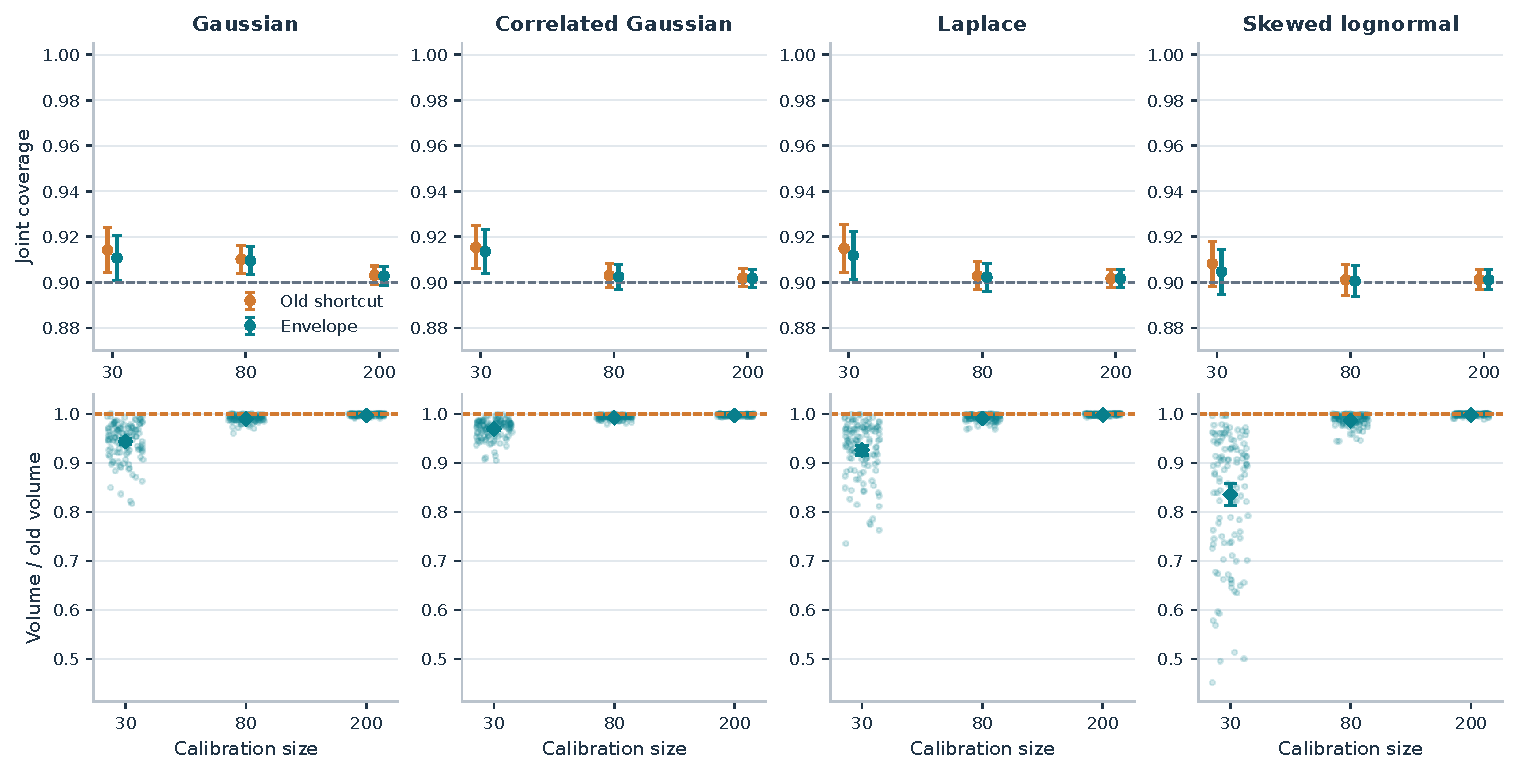
\includegraphics[width=\linewidth]{abs_main.pdf}
\caption{\textbf{Valid size reduction across four noise laws.} Six outcomes,
120 independent fitted trials per panel location, target 0.9. Top: mean joint
coverage with 95\% Monte Carlo intervals. Bottom: all paired outcome-volume
ratios (faint dots), their means (diamonds), and intervals. The dashed ratio
line marks equality. The shared vertical scale prevents small gains in one
family from appearing larger than substantial gains in another. All 1,440
volume pairs are finite.}
\label{fig:absolute}
\end{figure}

Across the four distributions, the average paired volume reduction is 8.13\%
at $n=30$, 1.03\% at $n=80$, and 0.27\% at $n=200$. Gains diminish as the
candidate contributes less to augmented calibration statistics. This is an
observed trend on this grid, not a proven monotonicity in $n$.
Skewed noise produces the largest small-sample reductions and appreciable
between-trial variation. Every observed ratio remains below one.

\begin{table}[H]\centering\small
\begin{tabular}{llrrrr}
\toprule
Scores & Noise & Old cov. & Env. cov. & Reduction & Pairs\\
\midrule
Absolute & Gaussian & 0.9102 & 0.9096 & $1.05\pm 0.12\%$ & 120\\
Capped CQR & Gaussian & 0.9062 & 0.9060 & $0.22\pm 0.04\%$ & 120\\
Absolute & Correlated Gaussian & 0.9030 & 0.9024 & $0.77\pm 0.07\%$ & 120\\
Capped CQR & Correlated Gaussian & 0.9052 & 0.9050 & $0.19\pm 0.03\%$ & 120\\
Absolute & Laplace & 0.9029 & 0.9023 & $0.92\pm 0.12\%$ & 120\\
Capped CQR & Laplace & 0.9047 & 0.9045 & $0.33\pm 0.05\%$ & 120\\
Absolute & Skewed lognormal & 0.9011 & 0.9006 & $1.37\pm 0.22\%$ & 120\\
Capped CQR & Skewed lognormal & 0.8997 & 0.8995 & $0.46\pm 0.07\%$ & 120\\
\bottomrule
\end{tabular}

\caption{\textbf{A common calibration-size comparison.} Six outcomes,
$n=80$, target 0.9. Reduction is $100(1-\overline{V_{\rm env}/V_{\rm old}})$;
the $\pm$ term is its 95\% Monte Carlo interval half-width. Pairs count
finite-volume comparisons. Capped CQR is included for direct comparison with
the next section. A point estimate just below 0.9 is possible under Monte
Carlo variation; the guarantee concerns the population experiment.}
\label{tab:common}
\end{table}

\clearpage
\section{Capped quantile residuals: the same theorem, additional edge cases}
\begin{figure}[H]\centering
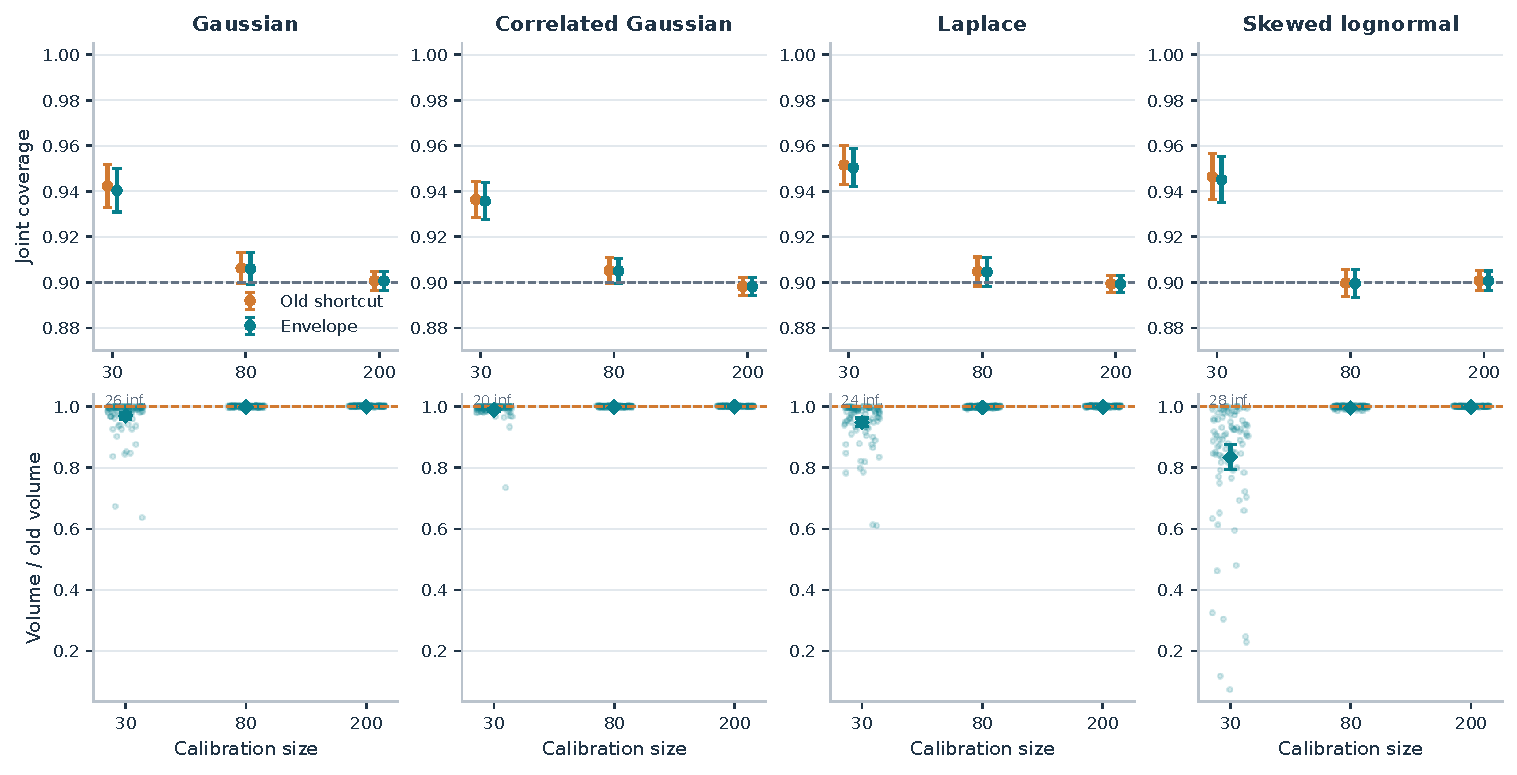
\includegraphics[width=\linewidth]{cap_main.pdf}
\caption{\textbf{Capped CQR isolates the envelope refinement.} Both methods
receive exactly the same capped calibration residuals and fitted base
intervals. Coverage includes infinite-region trials; bottom-row ratios are
restricted to finite pairs. The labels ``inf.'' count excluded pairs with an
infinite old volume. The envelope itself may be finite in such a pair, so the
finite-pair gain omits that improvement. All axes and uncertainty conventions
match Figure~\ref{fig:absolute}.}
\label{fig:capped}
\end{figure}

At $n=80$ the mean reductions range from 0.19\% to 0.46\%
(Table~\ref{tab:common}). These are consistent gains from the construction
alone, and they are considerably smaller than many signed-versus-capped gains.
Keeping the residual representation fixed makes the interpretation precise.

At $n=30$, the old shortcut has infinite volume in 98 of 480 trials
(20.4\%); the capped envelope does so in 88 (18.3\%). In 87 of these
small-sample trials, at least one capped coordinate has zero calibration
variance. Both methods then use the same explicitly documented whole-domain
fallback. Additional infinities can arise when the linked threshold reaches
the finite range limit of the self-score. No infinite trial is replaced by a
large plotting constant. Neither method has an infinite volume at $n=80$ or
$n=200$ in this primary grid.

\takeaway{\textbf{Read size and coverage together.} Capping creates a mass at
zero. Small-sample fallback can make coverage conservative and mean volume
infinite. Report the infinity rate next to finite-pair efficiency; the latter
does not estimate unconditional expected volume.}

\clearpage
\section{Uniformity and coordinate-by-coordinate comparisons}
\begin{figure}[H]\centering
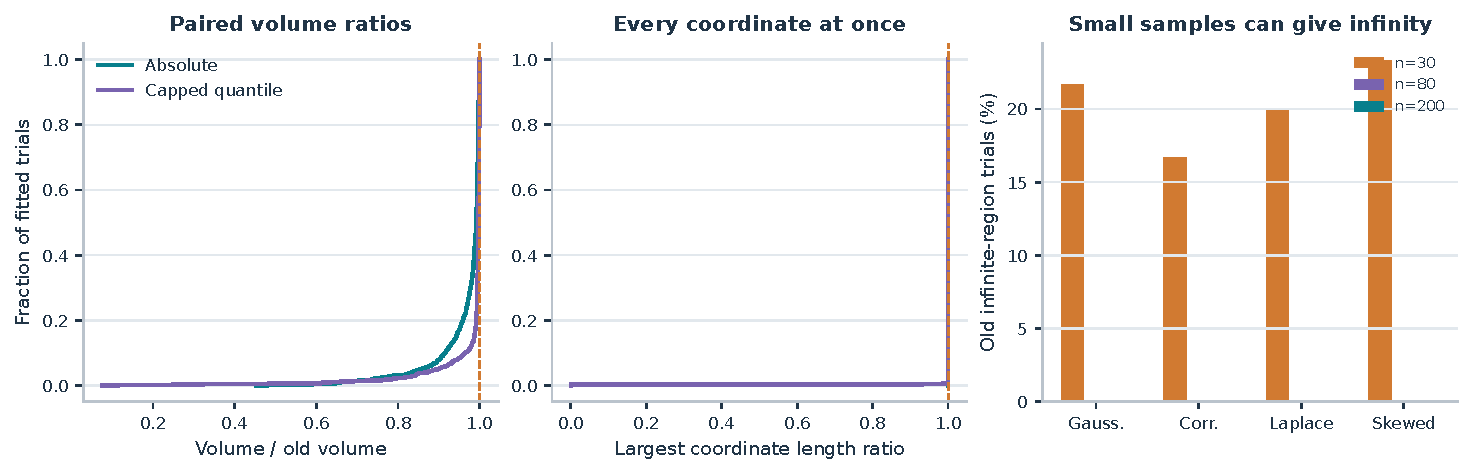
\includegraphics[width=\linewidth]{uniformity.pdf}
\caption{\textbf{The full paired distribution, not just its mean.} The first
two panels pool the primary grid: 1,440 finite absolute pairs and 1,342 finite
capped pairs. For each trial, the second panel takes the \emph{largest} of the
six coordinate length ratios, so a value above one would expose a coordinate
violation. Many coordinates coincide to numerical precision. The final panel
reports old-method infinity frequencies rather than hiding these trials in
the ratio distribution. A finite empirical audit supplements the pathwise
proof; it does not replace it.}
\label{fig:uniformity}
\end{figure}
\begin{figure}[H]\centering
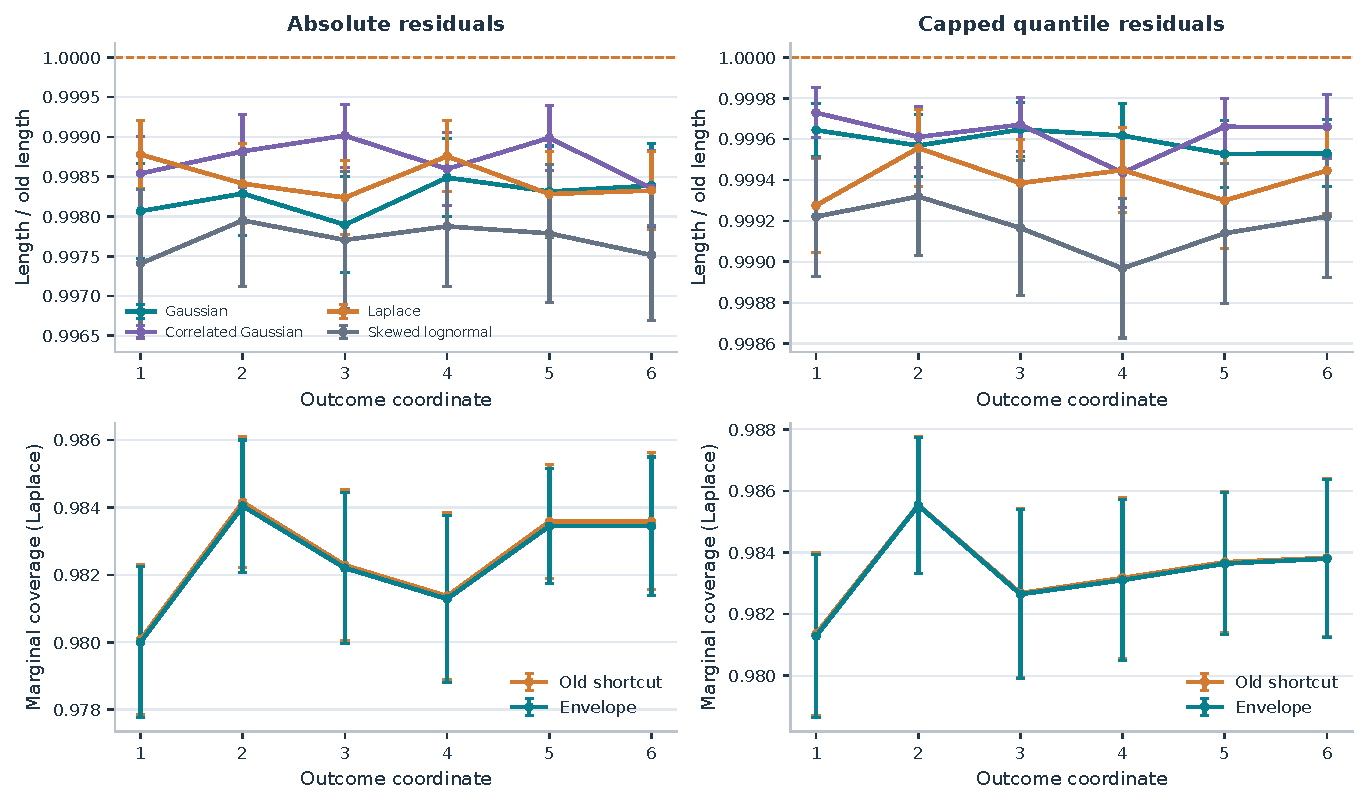
\includegraphics[width=.96\linewidth]{coordinate_comparison.pdf}
\caption{\textbf{Shorter in each coordinate, with coverage still visible.}
Top: paired mean length ratios and 95\% Monte Carlo intervals for all four
families at $n=80$, $d=6$. Bottom: marginal coverages for the Laplace study,
computed on the same trials. A high marginal coverage is not a substitute for
joint coverage; the latter is reported separately. Normalization by the old
length removes arbitrary outcome-unit differences.}
\label{fig:coordinate}
\end{figure}

The largest finite volume ratios are 0.999968 (absolute) and 0.999992 (capped).
Maximum coordinate ratios are within $2\times10^{-13}$ of one; these
near-equalities are not practically meaningful strict gains. Both same-score
comparisons pass on all 2,400 fitted trials, including common fallback cases.

\clearpage
\section{Coverage targets and volumes in outcome units}
\begin{figure}[H]\centering
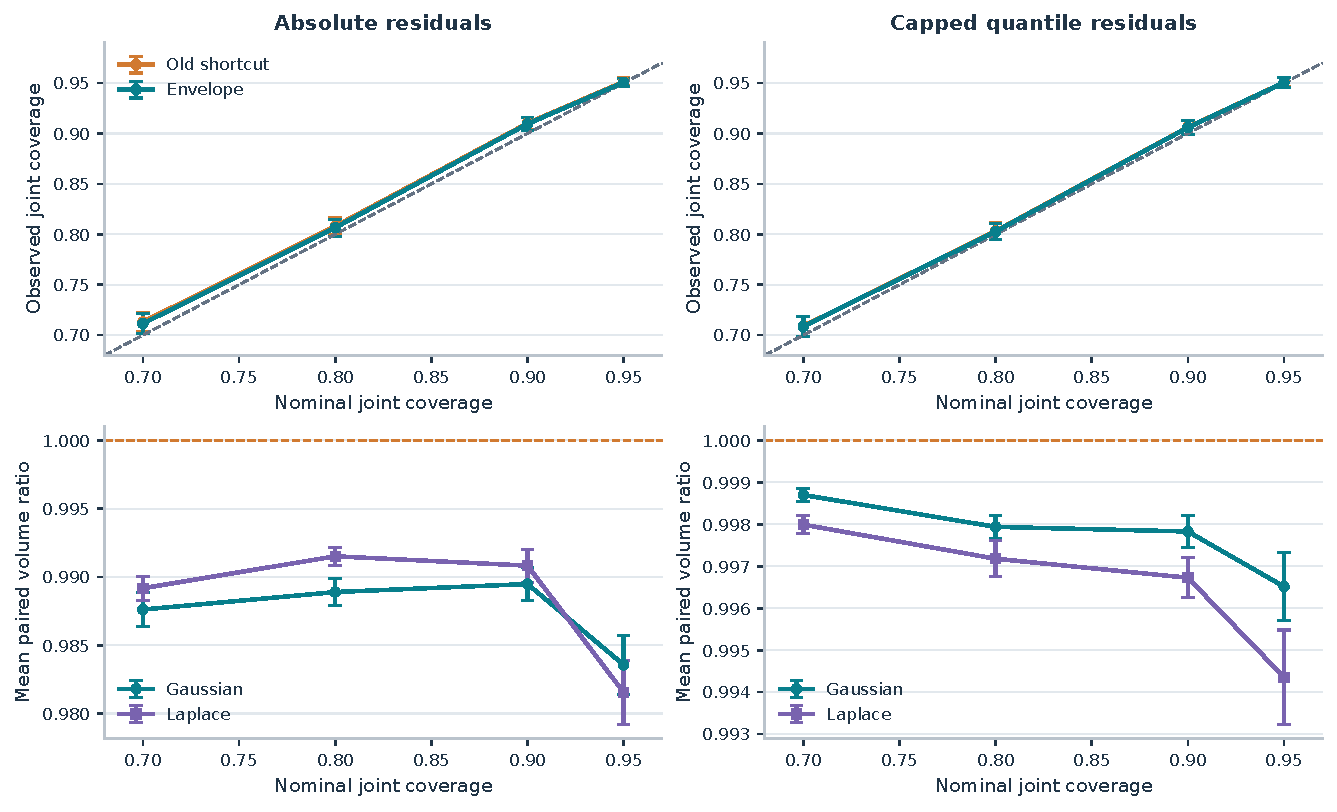
\includegraphics[width=.96\linewidth]{alpha_sweep.pdf}
\caption{\textbf{Changing the target does not change the comparison's
meaning.} At $n=80$, $d=6$, base miscoverage stays fixed at 0.1 while the
simultaneous target varies. Top: Gaussian joint coverage versus nominal
coverage, with the identity line. Bottom: paired volume ratios for Gaussian
and Laplace noise. The four target values use 120 independently fitted trials
each; the 0.9-target trials are the primary-grid data already shown, not extra
replications. Error bars are pointwise 95\% Monte Carlo intervals.}
\label{fig:alpha}
\end{figure}

\begin{table}[H]\centering\small
\begin{tabular}{llrr}
\toprule
Scores & Noise & Old mean volume & Envelope mean volume\\
\midrule
Absolute & Gaussian & 796235.2 & 787770.3\\
Capped CQR & Gaussian & 613944.2 & 612547.1\\
Absolute & Correlated Gaussian & 287799.9 & 285667.6\\
Capped CQR & Correlated Gaussian & 293560.1 & 292957.4\\
Absolute & Laplace & 2012805.1 & 1993559.9\\
Capped CQR & Laplace & 2093510.5 & 2085515.1\\
Absolute & Skewed lognormal & 3924120.3 & 3869557.1\\
Capped CQR & Skewed lognormal & 2099168.0 & 2087665.9\\
\bottomrule
\end{tabular}

\caption{\textbf{Volumes on the original outcome scale.} Arithmetic mean
six-dimensional volumes at $n=80$, corresponding to Table~\ref{tab:common}.
All pairs here are finite. Multiplying the six outcome lengths gives large
numbers even when coordinate changes are small. The ratio of these displayed
means generally differs from the mean paired ratio used in the plots.}
\label{tab:volumes}
\end{table}

Joint nominal coverage and base marginal coverage are different quantities.
For independent outcomes, even exactly fitted 90\% marginal intervals would
have joint coverage $0.9^6=0.5314$. This calculation explains why calibration
often expands the base intervals; the fitted toy's actual base coverage is
measured from data and need not equal this idealized value.

\clearpage
\section{Signed quantile residuals: separate the sources of improvement}
\begin{figure}[H]\centering
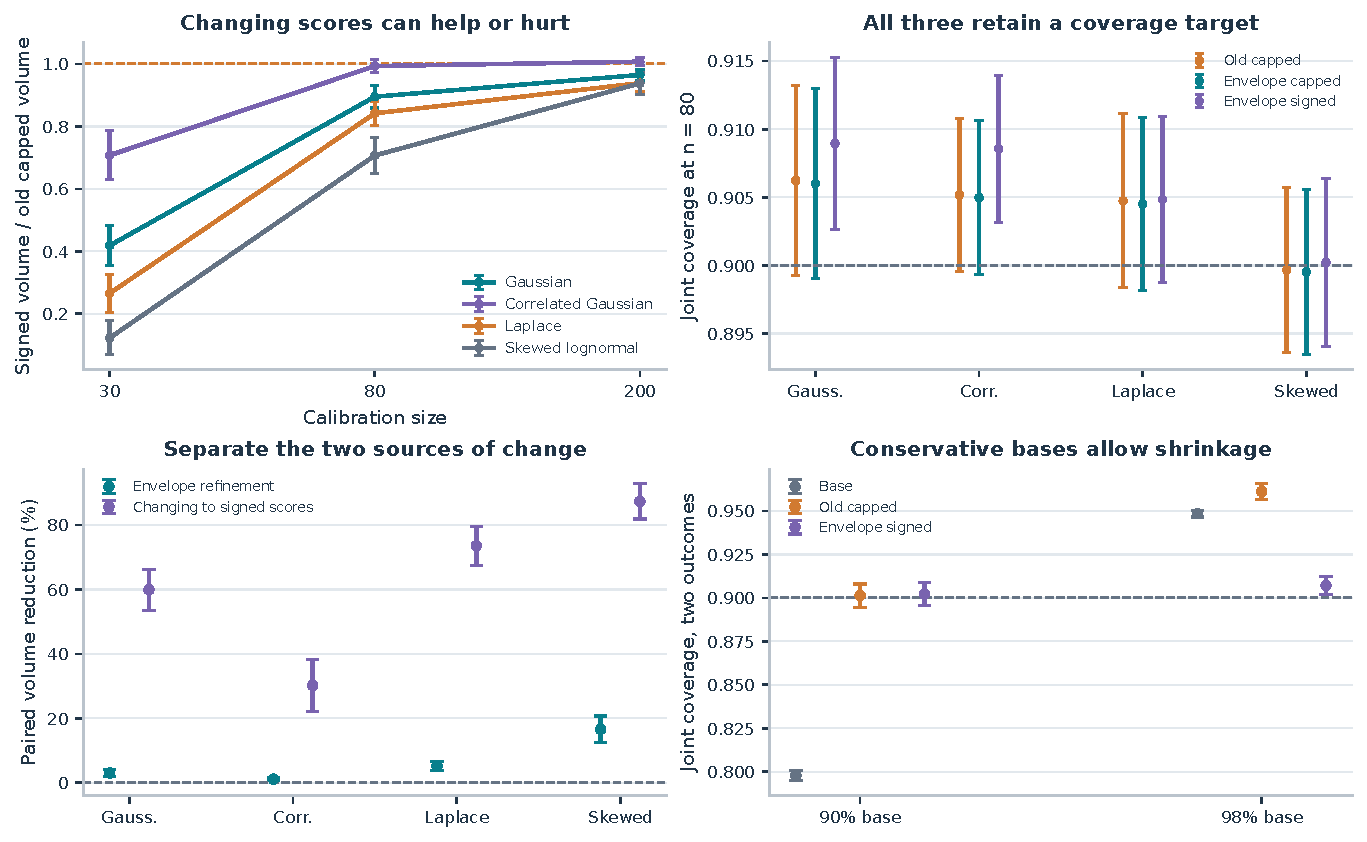
\includegraphics[width=\linewidth]{signed_comparison.pdf}
\caption{\textbf{A score change is not the same as an envelope refinement.}
Top left: signed-envelope / old-capped paired volume ratios on finite pairs;
crossing one means the signed version is larger. Top right: all-trial joint
coverage at $n=80$. Bottom left: at $n=30$, the two comparisons are
envelope-capped / old-capped and envelope-signed / envelope-capped, each using
its own finite-pair denominator set. Their reductions are not additive.
Bottom right: two-outcome Gaussian toys with 90\% and 98\% fitted marginal
bases, both calibrated to a 90\% joint target. All error bars are 95\%
Monte Carlo intervals across fitted trials.}
\label{fig:signed}
\end{figure}

The signed envelope is smaller on average than the old capped shortcut in
many configurations: at $n=80$, the finite-pair mean reductions are 10.49\%
(Gaussian), 0.68\% (correlated Gaussian), 15.83\% (Laplace), and 29.32\%
(skewed lognormal). Much of this change comes from retaining signed residuals,
not from tightening the same capped construction. The particularly large
small-$n$ gains are also sensitive to capped-score scale degeneracy and
heavy-tailed finite volumes; the finite-pair conditioning must be retained.

There is no samplewise signed-versus-capped superiority: the signed envelope
has larger volume in 359 of the 1,342 finite primary-grid comparisons, and the
largest observed ratio is 2.081. For correlated Gaussian noise at $n=200$,
its mean ratio is 1.007, with 95\% interval $[0.995,1.020]$.
This mean is statistically compatible with equality; the individual larger
regions already rule out uniform samplewise containment.

\takeaway{\textbf{What is proved for signed scores?}
$C_{\rm full,raw}\subseteq C_{\rm env,raw}\subseteq C_{\rm GWC,raw}$
and marginal joint coverage at least the target. The comparison to a capped
old shortcut is empirical and changes the full-conformal reference set.}

\clearpage
\section{One test input: expansion, contraction, and a concrete exception}
\begin{figure}[H]\centering
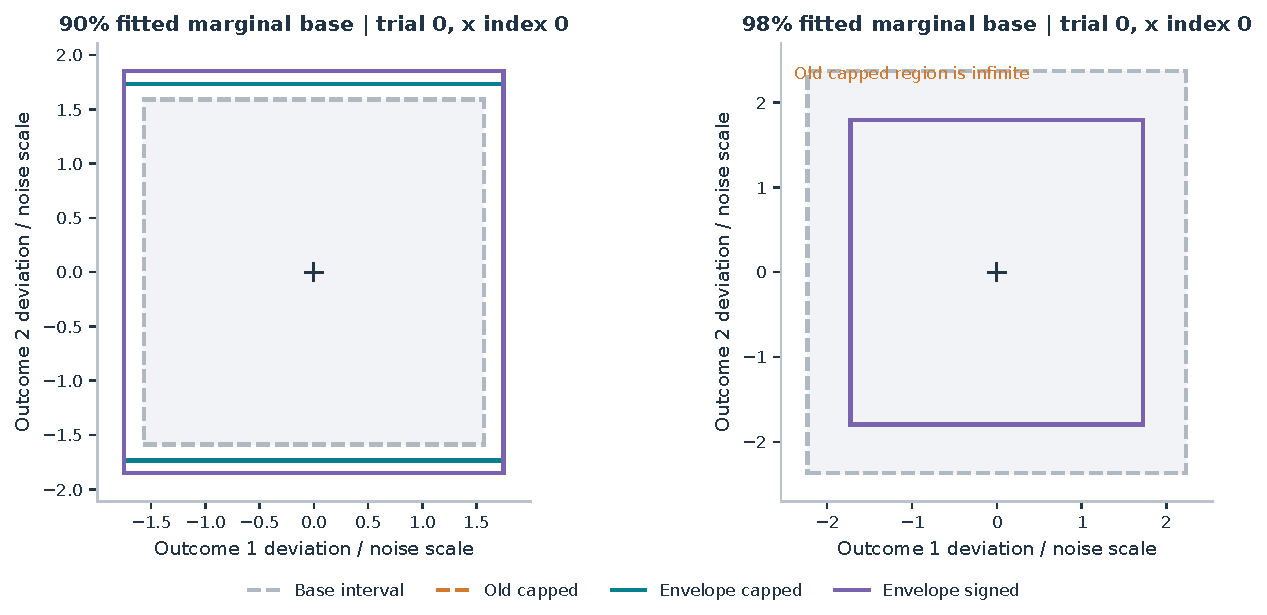
\includegraphics[width=\linewidth]{signed_geometry.pdf}
\caption{\textbf{Fixed-input signed geometry, without selecting a favorable
trial.} Both panels use trial 0 and test input 0 from the prespecified
two-outcome Gaussian studies. Coordinates are centered at the fitted
quantile midpoint and normalized by the DGP coordinate scales. Left: a 90\%
base must expand, and the signed envelope extends farther along outcome 2
than the capped construction. Right: a conservative 98\% base contracts
under signed calibration; both capped methods are infinite on this trial.
The unbounded regions are stated explicitly and are not drawn as finite boxes.}
\label{fig:signedgeometry}
\end{figure}

In the left panel, normalized outcome-2 half-widths are 1.735 for the old
capped shortcut and 1.851 for the signed envelope. This fixed example makes
the absence of signed-versus-capped containment tangible. In the right panel,
the base half-widths $(2.230,2.368)$ contract to $(1.723,1.792)$.

Across all 120 conservative-base trials, the signed envelope has joint
coverage 0.9071 and mean outcome area 52.37, versus base coverage 0.9485 and
area 62.53. The ratio of these mean areas implies a 16.25\% reduction relative
to the uncalibrated base; it is \emph{not} a paired reduction relative to the
old shortcut. Both capped methods have infinite volume in 29/120 trials.
Signed thresholds are negative in 88.75\% of test-coordinate evaluations,
averaged over trials. The 90\%-base study instead has signed coverage 0.9022
and needs expansion in most coordinates.

\paragraph{A useful invariance check.}
For a fixed coordinate shift $h_j$, shifting every calibration score and the
test-domain endpoint by $-h_j$ shifts the exact envelope threshold by $-h_j$.
Indeed $m$ and $z$ shift together, $s$ is unchanged, and $F$ is unchanged.
Thus with a covariate-independent symmetric base of half-width $h$, raw scores
$|Y-\hat f|-h$ reproduce the absolute-envelope outcome intervals, up to numerical
roundoff. A constant shift alone cannot create an efficiency gain.
Our groupwise bases vary with the covariate, and capping is nonlinear, so this
invariance does not imply equality in the reported signed-versus-capped study.

\clearpage
\section{Computation: measured speed and its limits}
\begin{figure}[H]\centering
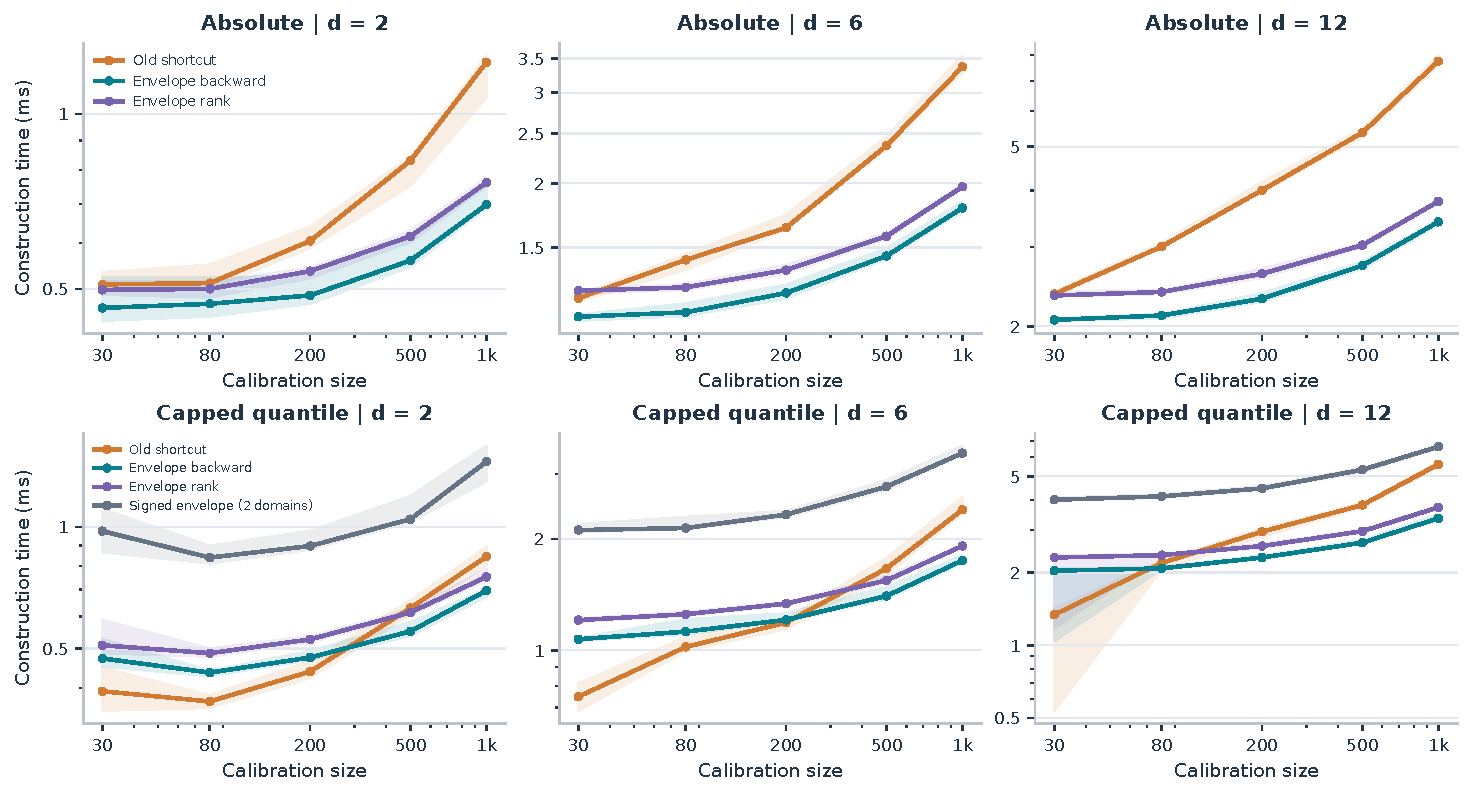
\includegraphics[width=\linewidth]{runtime.pdf}
\caption{\textbf{Serial region-construction timings.} Each $(n,d)$ cell uses
15 newly fitted Gaussian datasets. For each method, one untimed warmup is
followed by three timed calls in randomized method order; the dataset-level
statistic is their median. Lines show the median across datasets and bands
the interquartile range, not confidence intervals. Both axes are logarithmic;
panels use individual time ranges. Timing includes statistics,
sorting, and search, and excludes model fitting, evaluation, plotting, and
file I/O. Capped panels add raw signed envelope timing for both distinct
test-width domains using one calibration object. These are two predictions,
whereas a capped region is computed once for all test inputs.}
\label{fig:runtime}
\end{figure}

The absolute-envelope backward implementation is faster than the old
shortcut at all 15 plotted $(n,d)$ settings in this run; the ratios of median
old time to median envelope time range from 1.09 to 2.27. Capped comparisons
range from 0.66 to 1.67, so several small-sample cases favor the old shortcut.
Zero-scale fallbacks make some small capped cases particularly cheap. These
timings describe the supplied Python implementations on this Windows host,
not an algorithmic guarantee of uniform speed or a hardware-independent benchmark.

The envelope precomputes off-coordinate maxima in $O(nd)$ and uses $O(n)$
work per surface quantile. Unconditional backward search has worst-case
$O(dn^2+dn\log n)$ cost. The optional rank localization prunes a provably
failing suffix and returns identical bounds in the benchmark checks. Its
extra order statistic can cost more than it saves when backward search already
visits only one cell. Neither an unproved global binary-search predicate nor
full multidimensional cell enumeration is used here. The exact search proofs
and their qualified complexity bounds are retained in the appendix.

\clearpage
\section{Accuracy audit, reproduction, and scope}
\paragraph{Mathematical checks.}
The augmented scale uses the sample divisor $n$ on $n+1$ augmented observations;
the calibration $s_j^2$ uses divisor $n$ on $n$ observations. The signed inverse
keeps the sign of its argument. Coordinate suprema include endpoints and only
an admissible interior \emph{maximum}; negative suprema are not clamped to zero.
The conformal rank is $\lceil(n+1)(1-\alpha)\rceil$, with $+\infty$ when it
exceeds $n$. Candidate acceptance and cell boundaries are weak/closed.
Thresholds below the attainable domain mean an empty set, not a singleton.

The old global rule agrees algebraically with the exact GWC score for
nonnegative residuals before its positive jitter. The revised proof states
this connection explicitly. It also uses the minimum scale on the clipped
GWC interval when that interval does not contain the mean, rather than silently
substituting the unrestricted calibration scale. The code comparison retains
the old implementation's corrected tied-mean indexing and $10^{-10}$ positive
jitter. The report does not equate that floating-point executable to the
closed-cell mathematical comparator for arbitrary ties. New numerical
comparisons use tolerance $10^{-8}(1+|L_j^{\rm old}|)$.

\paragraph{Executed verification.}
The formula audit passed 150 augmented-standardization checks, 150 inverse
checks, 1,200 interval optimizations, 400 backward/exhaustive/rank agreements,
and 600 nonnegative comparisons. Of 33,651 candidate checks, all 10,683 full
conformal acceptances were retained. The protocol regression passed fresh-fit
checks, 500 atom-heavy draws (positive-scale cases checked), and 900 exact-zero
boundary checks. The new suite adds 2,400 pairs per same-score comparison,
450 benchmark search agreements, and the two geometry grids. These finite
checks support the supplied derivations, not a claim of exhaustive software
verification.
All 2,400 archive hashes and distinct training-data hashes were checked, and
every saved trial metric was recomputed. Full method bounds were also
recomputed on 60 prespecified archived trials; 120 constant-shift invariance
checks passed.

\paragraph{Reproducible outputs.}
The directory \path{envelope_method/report_revision/} contains
\path{design.json}, the deterministic generator and fitting code,
\path{trials.csv}, coordinate metrics, containment records, runtime observations,
summary tables, and figure code. Each of the 2,400 fitted trial archives stores
training/calibration/test features and outcomes, fitted coefficients, quantile
offsets, predictions, residuals, domains, and method bounds. The manifest records
SHA-256 digests. The master seed is 2026090917; configuration $k$, trial $b$
uses seed $2026090917+10000k+b$. Auxiliary benchmark and geometry seeds are
specified in the same runner. No historical synthetic results are reused in
the reported Monte Carlo summaries.

The README gives the exact simulation, figure, assembly, compilation,
environment, and rendering commands. Runtime reruns vary
with system load. Formula checks and the figure-generation grid are separate
from fitted-trial coverage experiments. No new full-LWC experiment is launched.

\paragraph{Scope of the evidence.}
This is a deliberately interpretable toy study, not a comprehensive model or
real-data benchmark. It tests four fixed DGP families and one lightweight
quantile-fitting scheme. Guarantees are marginal over calibration and a new
test observation, conditional on independent training; they are not conditional
coverage guarantees at every input. The report supports uniform \emph{weak
size improvement on identical nonnegative scores}; signed-score choices and
computational speed require the empirical qualifications above.

\clearpage
\appendix
\section{Setup and the conformal rank}
Condition throughout on an independently trained predictor and any training-only
choices. Let $(X^i,Y^i)_{i=1}^{n+1}$ be exchangeable and let
\[
 \E^i=\big(E_1(X^i,Y^i_1),\ldots,E_d(X^i,Y^i_d)\big)\in\R^d
\]
be coordinatewise nonconformity scores. The first $n$ residual vectors are
observed. Fix a test input $x$ and let $\evec=\E(x,y)$ denote a candidate
residual. Suppose its attainable coordinate values lie in
\[
 D_j(x)=[a_j(x),\infty)\cap\R,\qquad
 D(x)=\prod_{j=1}^d D_j(x),\qquad a_j(x)\in\R\cup\{-\infty\}.
\]
Here $a_j(x)$ is a known bound for the test residual, not an estimated bound on
the distribution. Calibration residuals at other covariates need not exceed
$a_j(x)$. A larger enclosing domain, including $D_j=\R$, is also valid.
Coordinatewise score sublevel sets must be intervals for the final prediction
set in outcome space to be a rectangle; validity itself does not require that.

Write $N=n+1$ and
\begin{equation}\label{eq:quantile}
 r=\lceil N(1-\alpha)\rceil,\qquad
 \Q(v_1,\ldots,v_n)=
 \begin{cases}v_{(r)},&r\le n,\\+\infty,&r=N.\end{cases}
\end{equation}
Use weak acceptance inequalities throughout. No jitter is needed, and ties are
allowed. If $v_i\le w_i$ for every $i$, then $\Q(v)\le\Q(w)$: for each real
$c$, at least as many $v_i$ as $w_i$ are at most $c$, so the ordered values have
the same ordering. This elementary monotonicity is used repeatedly below.

\begin{lemma}[Exchangeable rank]\label{lem:rank}
If $S^1,\ldots,S^N$ are exchangeable real scores, then
$\Pr\{S^N\le\Q(S^1,\ldots,S^n)\}\ge1-\alpha$.
\end{lemma}
\begin{proof}
Randomly break ties using independent continuous auxiliary variables. The rank
of the last score among the $N$ scores is uniform on $\{1,\ldots,N\}$ by
exchangeability. A rank at most $r$ implies the weak acceptance event in the
statement, including when tied values occur. Its probability is therefore at
least $r/N\ge1-\alpha$. If $r=N$, acceptance is automatic by
\eqref{eq:quantile}.
\end{proof}
This is the standard conformal rank argument; see \cite{shafer2008}.
The derivations of the envelope and its comparisons below are supplied here.

\section{Augmented standardization and its self-score link}
For each coordinate define
\begin{equation}\label{eq:observed}
 m_j=\frac1n\sum_{i=1}^n E^i_j,\qquad
 s_j^2=\frac1n\sum_{i=1}^n(E^i_j-m_j)^2.
\end{equation}
The divisor in $s_j^2$ is $n$, whereas the variance of the augmented $N$-point
sample below has divisor $N-1=n$. This distinction fixes all constants in the
link. Initially assume $s_j>0$ for every $j$; Section~\ref{sec:edges} supplies a
valid extension to degenerate calibration samples. Finite population moments
are unnecessary for the finite-sample argument.

For a candidate coordinate $z$, put $u=z-m_j$. The augmented mean is
\begin{equation}\label{eq:mu}
 \mu_j(z)=\frac{nm_j+z}{N}=m_j+\frac{u}{N}.
\end{equation}
Using $\sum_i(E^i_j-m_j)=0$ gives the full variance expansion
\begin{align}
 \sum_{i=1}^n(E^i_j-\mu_j(z))^2+(z-\mu_j(z))^2
 &=\sum_{i=1}^n\left(E^i_j-m_j-\frac{u}{N}\right)^2
      +\left(\frac{nu}{N}\right)^2\notag\\
 &=ns_j^2+\frac{nu^2}{N^2}+\frac{n^2u^2}{N^2}
  =ns_j^2+\frac{nu^2}{N}.\notag
\end{align}
Consequently
\begin{equation}\label{eq:sigma}
 \sigma_j(z)=\sqrt{s_j^2+\frac{(z-m_j)^2}{N}}.
\end{equation}
The basic coordinate transformation, its scalarization, and its candidate
self-score are respectively
\begin{align}
 F_j(t,z)&=\frac{t-\mu_j(z)}{\sigma_j(z)}
 =\frac{t-m_j-(z-m_j)/N}{\sqrt{s_j^2+(z-m_j)^2/N}},\label{eq:F}\\
 \Phi_{\zvec}(\tvec)&=\max_{j\le d}F_j(t_j,z_j),\label{eq:phi}\\
 g_j(e)&=F_j(e,e)
 =\frac{n(e-m_j)/N}{\sqrt{s_j^2+(e-m_j)^2/N}}.\label{eq:g}
\end{align}
Unlike a calibration-only fitted standardization, at the true test residual
these parameters are symmetric functions of all $N$ residual vectors.

\begin{lemma}[Signed inverse]\label{lem:link}
Let $T=n/\sqrt N$. The map $g_j:\R\to(-T,T)$ is strictly increasing, and
for finite $e$,
\begin{equation}\label{eq:linkequiv}
 g_j(e)\le c\quad\Longleftrightarrow\quad e\le\omega_j(c),
\end{equation}
where extended-real endpoints encode empty and unrestricted sublevels, and
\begin{equation}\label{eq:omega}
 \omega_j(c)=
 \begin{cases}
 -\infty,&c\le-T,\\[2pt]
 m_j+\displaystyle\frac{Ns_jc}{\sqrt{n^2-Nc^2}},&-T<c<T,\\[6pt]
 +\infty,&c\ge T.
 \end{cases}
\end{equation}
\end{lemma}
\begin{proof}
Direct differentiation gives
$g'_j(e)=(n/N)s_j^2\{s_j^2+(e-m_j)^2/N\}^{-3/2}>0$.
Its limits at $\pm\infty$ are $\pm T$, never attained at finite $e$.
For $|c|<T$, the equation $g_j(e)=c$, with $u=e-m_j$, yields
\[
 c\sqrt{s_j^2+u^2/N}=nu/N,
 \quad (n^2-Nc^2)u^2=N^2s_j^2c^2,
 \quad \operatorname{sign}(u)=\operatorname{sign}(c).
\]
Thus $u=Ns_jc/\sqrt{n^2-Nc^2}$. Keeping the sign condition is essential:
squaring alone would introduce a spurious root for negative $c$.
\end{proof}
The signed residual sublevel is $D_j(x)\cap(-\infty,\omega_j(c)]$.
There is no $\max\{0,\omega_j(c)\}$ in the signed link. If the upper endpoint
is below a finite $a_j(x)$, the sublevel is empty.

\section{The full conformal reference set}
For a candidate $\evec$ define
\begin{equation}\label{eq:oracle}
 Q_{\evec}=\Q\big(\Phi_{\evec}(\E^1),\ldots,
                          \Phi_{\evec}(\E^n)\big),\qquad
 C_{\mathrm{full}}(x)=\{y:\Phi_{\E(x,y)}(\E(x,y))\le Q_{\E(x,y)}\}.
\end{equation}
Equivalently, $y$ is accepted if $e_j\le\omega_j(Q_{\evec})$ for every $j$.
The threshold depends on the entire candidate, so this reference set need not
be rectangular or cheap to compute.

\begin{theorem}[Full conformal coverage]\label{thm:full}
Under exchangeability, $\Pr\{Y^{n+1}\in C_{\mathrm{full}}(X^{n+1})\}
\ge1-\alpha$.
\end{theorem}
\begin{proof}
At $\evec=\E^{n+1}$, augmenting the calibration sample gives precisely the full
exchangeable sample. The means and sample standard deviations of that sample
are invariant to permutation. Applying the same standardized maximum to each
of the $N$ observations therefore gives exchangeable scalar scores.
Lemma~\ref{lem:rank} proves the assertion. One need not assume that the scores
are independent of the fitted transformation.
\end{proof}

\section{Exact coordinate suprema and signed GWC}
For any nonempty interval $I=[\ell,u]\cap\R$, allowing infinite endpoints,
define
\begin{equation}\label{eq:psi}
 \psi_{j,I}(t)=\sup_{z\in I}F_j(t,z).
\end{equation}
Endpoint limits are included when the endpoint is infinite. Suppressing $j$,
differentiation of \eqref{eq:F} gives
\begin{equation}\label{eq:derivative}
 \frac{\partial F(t,z)}{\partial z}
 =-\frac{s^2+(t-m)(z-m)}{N\{s^2+(z-m)^2/N\}^{3/2}}.
\end{equation}
If $t>m$, the unique critical point is a maximum,
\begin{equation}\label{eq:critical}
 z^*(t)=m-\frac{s^2}{t-m},\qquad
 F(t,z^*(t))=\sqrt{\frac{(t-m)^2}{s^2}+\frac1N}.
\end{equation}
If $t<m$, its critical point is a minimum; if $t=m$, the function is decreasing.
Also $F(t,+\infty)=-1/\sqrt N$ and $F(t,-\infty)=1/\sqrt N$.
Thus the complete closed form is
\begin{equation}\label{eq:psiclosed}
 \psi_{j,I}(t)=\max\left\{
 F_j(t,\ell),F_j(t,u),
 \left.\sqrt{\frac{(t-m_j)^2}{s_j^2}+\frac1N}
 \ \right|\ t>m_j,\ z^*(t)\in I\right\}.
\end{equation}
The conditional entry is omitted when its condition fails, rather than replaced
by zero. Replacing it by zero would incorrectly inflate negative suprema.

The signed GWC score, quantile, and bounds are
\begin{align}
 \Phi_G(\tvec;x)&=\max_j\psi_{j,D_j(x)}(t_j)
                =\sup_{\zvec\in D(x)}\Phi_{\zvec}(\tvec),\label{eq:gwcscore}\\
 Q_G(x)&=\Q\big(\Phi_G(\E^1;x),\ldots,\Phi_G(\E^n;x)\big),\label{eq:gwcq}\\
 U_j(x)&=\omega_j(Q_G(x)),\quad G_j(x)=D_j(x)\cap(-\infty,U_j(x)],
 \quad G(x)=\prod_jG_j(x),\label{eq:G}\\
 \Cgwc(x)&=\{y:\E(x,y)\in G(x)\}.\label{eq:Cgwc}
\end{align}
For a finite lower endpoint $a_j$, \eqref{eq:psiclosed} uses $F_j(t,a_j)$,
$-1/\sqrt N$, and the critical maximum when $t>m_j$ and $z^*(t)\ge a_j$.
For $a_j=-\infty$ it simplifies to
\[
 \psi_{j,\R}(t)=
 \begin{cases}
 \sqrt{(t-m_j)^2/s_j^2+1/N},&t>m_j,\\
 1/\sqrt N,&t\le m_j.
 \end{cases}
\]

\begin{proposition}[GWC containment]\label{prop:gwc}
For every realized calibration sample and test input,
\[C_{\mathrm{full}}(x)\subseteq\Cgwc(x).\]
\end{proposition}
\begin{proof}
For a candidate in $D(x)$, $\Phi_{\evec}(\E^i)\le\Phi_G(\E^i;x)$ for every
$i$, whence $Q_{\evec}\le Q_G$. Full acceptance implies
$g_j(e_j)\le Q_{\evec}\le Q_G$, and Lemma~\ref{lem:link} gives $e_j\le U_j$.
\end{proof}
The dependence of $D(x)$ on the test input causes no difficulty: this is a
pathwise containment argument, not a claim that GWC calibration scores formed
using that input are exchangeable on their own.

\section{From full cells to surface envelopes}
Assume $G(x)$ is nonempty. For each coordinate, partition $G_j$ using its two
endpoints and the distinct calibration residuals strictly between them:
\[
 a_j=\eta_{j,0}<\eta_{j,1}<\cdots<\eta_{j,K_j}=U_j,
 \qquad I_{j,k}=[\eta_{j,k-1},\eta_{j,k}]\cap\R.
\]
There are at most $n+1$ cells. We deliberately use closed cells, a cover with
shared endpoints. This prevents boundary exclusions when residuals have atoms.
A singleton $G_j$ is represented by one singleton cell. Distinct interior
knots avoid zero-width duplicate cells. The proofs allow any finite ordered
interval cover, though Section~\ref{sec:binary} uses the calibration partition.

A full cell $\mathcal I_h=\prod_j I_{j,h_j}$ has exact local score
\[
 \Phi_h^{\mathrm{exact}}(\tvec)=
 \sup_{\zvec\in\mathcal I_h}\Phi_{\zvec}(\tvec)
 =\max_j\psi_{j,I_{j,h_j}}(t_j).
\]
Enumerating all $h$ costs up to $(n+1)^d$ cells. Instead fix only the $j$th
coordinate cell and let the others range over GWC:
\begin{align}
 H_j(\tvec)&=\max_{\ell\ne j}\psi_{\ell,G_\ell}(t_\ell),\label{eq:H}\\
 \overline\Phi_{j,k}(\tvec)&=
 \max\{\psi_{j,I_{j,k}}(t_j),H_j(\tvec)\}
 =\sup_{\substack{z_j\in I_{j,k}\\z_\ell\in G_\ell,\ \ell\ne j}}
       \Phi_{\zvec}(\tvec),\label{eq:surface}\\
 \overline Q_{j,k}&=\Q\big(\overline\Phi_{j,k}(\E^1),\ldots,
                              \overline\Phi_{j,k}(\E^n)\big).\label{eq:surfaceq}
\end{align}
Set $H_1=-\infty$ for $d=1$. Every transformation in these formulas is given
explicitly by \eqref{eq:psiclosed}. For $h_j=k$ we have the pointwise chain
\begin{equation}\label{eq:chain}
 \Phi_{\evec}\le\Phi_h^{\mathrm{exact}}\le\overline\Phi_{j,k}\le\Phi_G
 \quad\hbox{whenever }\evec\in\mathcal I_h.
\end{equation}
The envelope enlarges the candidate domain before taking the supremum. In
general a quantile of pointwise maxima is not the maximum of the corresponding
quantiles. Thus no equality with exact full-cell LWC is asserted.

Define the accepted coordinate piece and its upper endpoint by
\begin{align}
 A_{j,k}&=I_{j,k}\cap(-\infty,\omega_j(\overline Q_{j,k})],\label{eq:piece}\\
 B_{j,k}&=
 \begin{cases}
 \min\{\eta_{j,k},\omega_j(\overline Q_{j,k})\},&A_{j,k}\ne\varnothing,\\
 -\infty,&A_{j,k}=\varnothing.
 \end{cases}\label{eq:B}
\end{align}
For a finite lower endpoint, nonemptiness is exactly
$\omega_j(\overline Q_{j,k})\ge\eta_{j,k-1}$; a value $-\infty$ never
represents a finite residual. In particular, equality retains the singleton at
the cell's left endpoint. Let
\begin{equation}\label{eq:L}
 L_j=\max_{1\le k\le K_j}B_{j,k},\qquad
 R_{\mathrm{env}}(x)=D(x)\cap\prod_j(-\infty,L_j],\qquad
 \Cenv(x)=\{y:\E(x,y)\in R_{\mathrm{env}}(x)\}.
\end{equation}
If any coordinate has no accepted piece, return the empty set. Otherwise
$R_{\mathrm{env}}$ is the coordinatewise lower enclosure of the pieces; it may
fill gaps between them. It is not being identified with the exact local union.

\begin{theorem}[Signed envelope validity]\label{thm:valid}
Pathwise, $C_{\mathrm{full}}(x)\subseteq\Cenv(x)\subseteq\Cgwc(x)$.
Consequently $\Pr\{Y^{n+1}\in\Cenv(X^{n+1})\}\ge1-\alpha$.
\end{theorem}
\begin{proof}
Take $y\in C_{\mathrm{full}}(x)$. Proposition~\ref{prop:gwc} implies that its
residual $\evec$ belongs to $G(x)$. For each $j$, choose a covering cell
$I_{j,k}$ containing $e_j$. Every calibration observation satisfies
$\Phi_{\evec}(\E^i)\le\overline\Phi_{j,k}(\E^i)$. Quantile monotonicity and
full acceptance therefore yield
\[
 g_j(e_j)\le\max_\ell g_\ell(e_\ell)
 \le Q_{\evec}\le\overline Q_{j,k},
 \quad e_j\le\omega_j(\overline Q_{j,k}),
 \quad e_j\in A_{j,k},
 \quad e_j\le B_{j,k}\le L_j.
\]
This proves the first containment simultaneously for all coordinates without a
Bonferroni correction. Each nonempty $A_{j,k}$ lies in $G_j$, so $L_j\le U_j$,
which proves the second. The coverage statement follows from
Theorem~\ref{thm:full}.
\end{proof}

\section{Why it improves the old separated shortcut}\label{sec:dominance}
Here the comparison uses the \emph{same nonnegative calibration residuals},
test score function, level $\alpha$, and calibration partition, with $D_j=[0,\infty)$.
It does not compare signed residuals to capped or shifted residuals. Assume
$s_j>0$.

The mathematical old GWC transformation is the same exact supremum
$\max_j\psi_{j,[0,\infty)}(t_j)$ as \eqref{eq:gwcscore}. Its implementation
evaluates the endpoint at zero, the limit at infinity, and the stationary
point. For $t_j>m_j$, an admissible stationary point is exactly the maximum
in \eqref{eq:critical}; for $t_j<m_j$ the stationary point is a minimum and
cannot exceed both endpoints. Thus, in exact arithmetic and without jitter,
$G^{\mathrm{old}}=G$ for the same nonnegative scores and rank.
The implementation's nonnegative jitter can only enlarge the GWC quantile;
the theoretical comparison below is made with the unperturbed closed rules.
 Define the old GWC box $G^{\mathrm{old}}$ and
\begin{equation}\label{eq:oldconst}
 c_\ell=\inf_{z\in G^{\mathrm{old}}_\ell}\frac{\mu_\ell(z)}{\sigma_\ell(z)},
 \qquad r_\ell(h)=\inf_{z\in I^{\mathrm{old}}_{\ell,h}}\sigma_\ell(z).
\end{equation}
For nonnegative residuals $m_\ell\ge0$ and
$G^{\mathrm{old}}_\ell=[0,U^{\mathrm{old}}_\ell]$. Differentiating
$\mu(z)/\sigma(z)$ gives
\[
 \frac{d}{dz}\frac{\mu(z)}{\sigma(z)}
 =\frac{s^2-m(z-m)}{N\sigma(z)^3}.
\]
Its interior critical point, when present, is a maximum. Thus
\[
 c_\ell=\min\left\{\frac{\mu_\ell(0)}{\sigma_\ell(0)},
                      \frac{\mu_\ell(U^{\mathrm{old}}_\ell)}
                           {\sigma_\ell(U^{\mathrm{old}}_\ell)}\right\},
\]
with the second expression interpreted as $1/\sqrt N$ at infinity, and
\[
 r_\ell(h)=\sqrt{s_\ell^2+
   \operatorname{dist}(m_\ell,I^{\mathrm{old}}_{\ell,h})^2/N}.
\]
The old separated score on a full cell is
\[
 \Phi_h^{\mathrm{sep}}(\tvec)
 =\max_\ell\{t_\ell/r_\ell(h_\ell)-c_\ell\},\qquad \tvec\ge0.
\]
Let $p_\ell=\operatorname{proj}_{G^{\mathrm{old}}_\ell}(m_\ell)$ and
$\bar s_\ell=\sigma_\ell(p_\ell)=\inf_{z\in G^{\mathrm{old}}_\ell}\sigma_\ell(z)$.
If $m_\ell\in G^{\mathrm{old}}_\ell$, then $p_\ell=m_\ell$ and
$\bar s_\ell=s_\ell$. Otherwise $\bar s_\ell$ is the minimum scale on the
clipped domain, which need not equal $s_\ell$.
Choose each off-coordinate old cell to contain $p_\ell$. Whenever the old
mean cell intersects GWC it has this property after clipping. Its minimum
scale is therefore $\bar s_\ell$. The old row score is
\begin{equation}\label{eq:oldrow}
 \Phi^{\mathrm{old}}_{j,k}(\tvec)=
 \max\left\{\frac{t_j}{r_j(k)}-c_j,
             \max_{\ell\ne j}\left(\frac{t_\ell}{\bar s_\ell}-c_\ell\right)\right\}.
\end{equation}
Its quantile and clipped coordinate pieces define $L_j^{\mathrm{old}}$ as
in \eqref{eq:surfaceq}--\eqref{eq:L}, using the old cells. If the old mean
cell is unavailable, the manuscript shortcut returns its GWC box.

\begin{lemma}[Pointwise score domination]\label{lem:domination}
For $\tvec\ge0$ and the same GWC box and cells,
$\overline\Phi_{j,k}(\tvec)\le\Phi^{\mathrm{old}}_{j,k}(\tvec)$.
\end{lemma}
\begin{proof}
For $z\in I_{j,k}$, $\sigma_j(z)\ge r_j(k)>0$ and
$\mu_j(z)/\sigma_j(z)\ge c_j$. Nonnegativity gives
\[
 F_j(t_j,z)=\frac{t_j}{\sigma_j(z)}-\frac{\mu_j(z)}{\sigma_j(z)}
 \le\frac{t_j}{r_j(k)}-c_j.
\]
Taking the supremum proves the active-coordinate inequality. For $\ell\ne j$
and $z\in G_\ell$, $\sigma_\ell(z)\ge\bar s_\ell$, so similarly
$F_\ell(t_\ell,z)\le t_\ell/\bar s_\ell-c_\ell$. Take the off-coordinate suprema
and then the maximum. Both steps explicitly use $t_\ell\ge0$; reversing its
sign reverses the comparison of the scale terms.
\end{proof}

\begin{theorem}[Uniform weak improvement over the old shortcut]\label{thm:dom}
Under the preceding conditions, with closed-cell and weak-acceptance conventions
for both constructions,
\[
 \Cenv(x)\subseteq C_{\mathrm{old}}(x),\qquad
 L_j\le L_j^{\mathrm{old}}\quad(j\le d)
\]
whenever both coordinate bounds represent nonempty sets. The set containment
also holds when the envelope is empty or when the old shortcut falls back to
GWC. In particular, each outcome interval and the resulting rectangular volume
are weakly smaller, while finite-sample coverage remains at least $1-\alpha$.
\end{theorem}
\begin{proof}
Lemma~\ref{lem:domination} and quantile monotonicity give
$\overline Q_{j,k}\le Q^{\mathrm{old}}_{j,k}$. The signed link is increasing,
so each accepted envelope piece is contained in its corresponding old piece.
Taking coordinatewise suprema yields $L_j\le L_j^{\mathrm{old}}$. Taking score
sublevel sets preserves containment in outcome space. On an old GWC fallback
sample, Theorem~\ref{thm:valid} gives the result directly.
\end{proof}
The proof also works if the envelope's GWC box is a subset of the old box and
its cells refine the old cells: each supremum is then over a smaller domain.
Thus a harmless outward rounding in the old GWC computation does not reverse
the mathematical comparison.

\paragraph{What the statement does and does not compare.}
The old manuscript uses some strict cell tests and assumes distinct residuals;
the present note specifies a closed version to cover atoms as well. A literal
comparison to code with a different tie policy requires numerical checking or
harmonizing those policies; it is not justified by ignoring endpoints.
The repository's old implementation also adds positive numerical jitter.
The mathematical theorem is about the explicitly defined rules, not arbitrary
floating-point perturbations. The paired experiment audit separately compares
the actual implementations. During that audit, capped CQR scores exposed a
specific bug in the former implementation: \texttt{argmax} selected the first
tied zero below the mean, which could select a $[0,0]$ cell not containing the
strictly positive mean. The off-coordinate scale then exceeded $s_\ell$, so
\eqref{eq:oldrow} no longer described that code. Selecting the last value at
or below the mean (right-sided insertion rank) restores a mean-containing cell.
All six saved failing examples satisfy containment after this correction;
additional atom-heavy regression tests cover the same issue. Thus the theorem
compares the mathematical old shortcut, including this necessary tie fix,
and does not claim dominance over the buggy historical executable.
The theorem is a containment result, not a claim
that the envelope has higher coverage than a larger old set. Strict size
improvement need not occur. Exact full-ratio cell LWC can be tighter than the
surface envelope, and CQHR has a different scalarization; neither is dominated
by this argument.

\section{Computation and a justified search rule}
Compute $m,s$ and the GWC scores in $O(nd)$ operations. Sort the distinct
calibration coordinates in $O(dn\log n)$. Precompute
$V_{i\ell}=\psi_{\ell,G_\ell}(E^i_\ell)$ and all
$H_{ij}=\max_{\ell\ne j}V_{i\ell}$ in $O(nd)$ using left and right cumulative
maxima. Each surface quantile then requires $O(n)$ arithmetic and an order
statistic selection, with no factor of $d$ inside the surface search.

\begin{lemma}[Rightmost surviving cell]\label{lem:backward}
For any ordered interval cover, the largest $B_{j,k}$ is the endpoint of the
rightmost nonempty $A_{j,k}$. Thus scanning from $K_j$ downwards and stopping at
the first nonempty piece computes $L_j$ exactly, without a monotone predicate.
\end{lemma}
\begin{proof}
If cell $k$ survives and $h<k$, then
$B_{j,h}\le\eta_{j,h}\le\eta_{j,k-1}\le B_{j,k}$ whenever $h$ survives.
An empty piece cannot increase the maximum. All cells to the right have already
been checked and are empty.
\end{proof}
The worst-case cost is $O(dn^2+dn\log n)$, and the actual search cost is
$O(n\sum_j M_j)$ when $M_j$ cells are inspected. The implementation records
these counts. This proof does not claim that the values $B_{j,k}$ are monotone:
they drop to the empty sentinel after a failure.

\subsection{A range where binary search is proved}\label{sec:binary}
For $n>1$ put $b_j=m_j-s_j/\sqrt{n-1}$. We prove a stronger search fact than
the usual restriction to cells above the empirical mean, but make no
unconditional prefix claim for the cells below $b_j$.

\begin{lemma}[Rank-count predicate above $b_j$]\label{lem:binary}
Consider a calibration-partition cell $I_{j,k}=[\ell,u]$ with finite
$\ell>b_j$ and $u>\ell$. Set $h_i=H_j(\E^i)$. Then
\begin{equation}\label{eq:rankpredicate}
 A_{j,k}\ne\varnothing\quad\Longleftrightarrow\quad
 \#\{i:E^i_j<\ell,\ h_i<g_j(\ell)\}<r.
\end{equation}
Consequently the survival predicate is a true prefix followed by a false suffix
on these cells, and binary search is valid on this part of the partition.
\end{lemma}
\begin{proof}
First $g_j(\ell)>-1/\sqrt N$ is equivalent to $\ell>b_j$ by
\eqref{eq:g}. For fixed $t=\ell$, \eqref{eq:derivative} shows that
$F_j(\ell,z)$ has either no interior maximum or is decreasing for $z\ge\ell$.
Its supremum over $[\ell,\infty)$ is the larger of $g_j(\ell)$ and
$-1/\sqrt N$, hence is $g_j(\ell)$. More explicitly, if $\ell<m_j$ the
interior critical point is a minimum; if $\ell\ge m_j$ the derivative is
negative on this half-line.

If $t<\ell$, then $F_j(t,z)<F_j(\ell,z)$ at every finite $z$, and its limit
at infinity is strictly below $g_j(\ell)$. Continuity, including that limit,
therefore implies $\psi_{j,I_{j,k}}(t)<g_j(\ell)$. If $t=\ell$, the supremum
equals $g_j(\ell)$. If $t>\ell$, evaluating at $z=\ell$ already gives a value
strictly larger than $g_j(\ell)$. It follows that the $i$th surface score is
strictly below $g_j(\ell)$ exactly when both inequalities inside the count in
\eqref{eq:rankpredicate} hold. Its $r$th order statistic is at least
$g_j(\ell)$ exactly when fewer than $r$ scores are strictly below this value.
Link inversion proves the equivalence. As $\ell$ increases, $g_j(\ell)$
increases, so the counted sets are nested and their cardinalities cannot decrease.
\end{proof}
In fact, the proof of the rank predicate uses only $z\ge\ell$ and the left
endpoint; no sign assumption is placed on the calibration residuals.
One can check the top cell first, use binary search on the cells with left
endpoint above $b_j$, and scan backwards below that range only if no upper
cell survives. This has $O(dn\log n)$ search cost when every coordinate boundary
is found in the proved range, with the unconditional backward bound otherwise.
Observed prefix behavior outside the proved range must not be substituted for
a proof. The initial reference implementation uses unconditional backward search
so its correctness does not depend on this optional acceleration.

\subsection{Direct order-statistic localization}\label{sec:ranklocal}
Binary search is not necessary in the certified range. For each coordinate set
\[
 W_{ij}=\max\{E^i_j,\,\omega_j(H_j(\E^i))\},\qquad
 T_j=W_{(r),j},
\]
where $W_{(r),j}$ is the $r$th order statistic, with the same infinite-rank
convention. The inverse is evaluated separately at each off-coordinate score;
it is not the inverse of an aggregate quantile.
\begin{proposition}[One-order-statistic localization]\label{prop:ranklocal}
For a nondegenerate cell with left endpoint $\ell>b_j$,
\[
 A_{j,k}\ne\varnothing\quad\Longleftrightarrow\quad \ell\le T_j.
\]
In particular every cell with left endpoint exceeding
$\max\{b_j,T_j\}$ can be discarded without evaluating a surface quantile.
\end{proposition}
\begin{proof}
The extended inverse convention gives
$h_i<g_j(\ell)\Longleftrightarrow\omega_j(h_i)<\ell$ even when
$h_i$ is outside the open range of $g_j$. Hence
\[
 \{E^i_j<\ell,\ h_i<g_j(\ell)\}
 =\{\max(E^i_j,\omega_j(h_i))<\ell\}=\{W_{ij}<\ell\}.
\]
There are fewer than $r$ such values exactly when $W_{(r),j}\ge\ell$.
Apply Lemma~\ref{lem:binary}. The discarded cells are all in that lemma's
range, so this pruning makes no claim about the remaining lower cells.
\end{proof}
Select $T_j$ in $O(n)$ time and find the last partition left endpoint at or
below $\max\{b_j,T_j\}$ by insertion search in $O(\log n)$ time. Start the
unconditional backward scan there. If this cell has left endpoint above $b_j$,
it is the rightmost survivor and only its surface quantile is needed to compute
the actual clipped endpoint $B_{j,k}$. The endpoint is generally \emph{not}
$T_j$: the order statistic localizes the cell, after which
\eqref{eq:surfaceq}--\eqref{eq:L} still determine its boundary.
If the candidate cell is below the certified range, continue backward normally.
Thus search costs $O(nd+d\log n)$ when all coordinate boundaries lie in the
certified range, after sorting and off-coordinate preprocessing, with the
unconditional worst-case bound otherwise. The optional implementation
\texttt{search="rank"} uses this pruning and an outward numerical guard near
ties. It need not be faster on typical samples: a backward scan that already
checks one cell avoids the extra transformed order statistic.

\section{Outcome intervals, signed improvements, and edge cases}\label{sec:edges}
For absolute residuals $E_j(x,y)=|y-\hat f_j(x)|$, $a_j=0$ and the prediction
interval is $[\hat f_j(x)-L_j,\hat f_j(x)+L_j]$.
For ordered fitted quantiles $q^-_j(x)\le q^+_j(x)$, signed CQR scores satisfy
\begin{align*}
 E_j(x,y)&=\max\{q^-_j(x)-y,\ y-q^+_j(x)\}\\
 &=\left|y-\frac{q^-_j(x)+q^+_j(x)}2\right|
                  -\frac{q^+_j(x)-q^-_j(x)}2,
 \qquad a_j(x)=-\frac{q^+_j(x)-q^-_j(x)}2.
\end{align*}
Consequently
\[
 E_j(x,y)\le L_j
 \Longleftrightarrow
 q^-_j(x)-L_j\le y\le q^+_j(x)+L_j,
 \qquad \operatorname{length}_j=(q^+_j-q^-_j)+2L_j.
\]
A negative $L_j$ shrinks the base interval. A bound below $a_j$ means an empty
interval, not a singleton created by clamping. A bound equal to $a_j$ gives
the singleton at the midpoint. Mixed signs across coordinates are allowed;
GWC inflation in one or all coordinates does not rule out local shrinkage.
The envelope's computations for one coordinate still depend on the other
coordinates through $H_j$, so a general sign-reflection shortcut is not implied.

\paragraph{Small calibration samples.}
If $r=N$, all conformal quantiles are $+\infty$ and the procedure returns the
entire attainable domain. An implementation must preserve this case, not
replace the quantile by the largest observed score.

\paragraph{Zero calibration variance.}
To extend the definition to all finite calibration samples, define the full
conformal reference scale to be the augmented sample standard deviation when
positive, and $1$ when the entire augmented coordinate is constant. This rule
is symmetric, so Theorem~\ref{thm:full} still holds. If any observed $s_j=0$,
the reference implementation returns the whole attainable domain, a valid
superset of that same reference set. Otherwise all proofs above apply.
This conservative fallback avoids division by zero; it can be costly for
heavily capped scores. The positive-score dominance theorem excludes these
samples because the unregularized old shortcut also lacks a positive scale.
A practical regularized variant could instead add a predetermined positive
ridge to every augmented variance symmetrically, but its comparison must then
be made to an old shortcut with matching regularization.

\paragraph{Infinity, empty boxes, and ties.}
If GWC is empty, return empty immediately. Infinite cell endpoints use the
limits in \eqref{eq:psiclosed}. An infinite upper coordinate makes volume
infinite unless some coordinate interval is empty or has zero length, in which
case rectangular Lebesgue volume is zero. Closed cells and weak inequalities
are maintained across calibration ties and candidate ties. The finite-sample
coverage guarantee is marginal over the calibration/test experiment; it is not
a guarantee conditional on the realized calibration sample or on every $x$.


\begin{thebibliography}{9}
\bibitem{shafer2008} G. Shafer and V. Vovk (2008).
A Tutorial on Conformal Prediction. \emph{Journal of Machine Learning Research}
9:371--421. \url{https://jmlr.org/papers/v9/shafer08a.html}.
\bibitem{romano2019} Y. Romano, E. Patterson, and E. J. Cand\`es (2019).
Conformalized Quantile Regression. \emph{Advances in Neural Information
Processing Systems} 32.
\url{https://proceedings.neurips.cc/paper/2019/hash/5103c3584b063c431bd1268e9b5e76fb-Abstract.html}.
\end{thebibliography}
\end{document}

